
\newcommand{\trillWidth}{101.6mm / 1.2}
\newcommand{\trillHeight}{21.5mm / 1.2}
\newcommand{\NumStrings}{6}
\newcommand{\StringWidth}{\trillWidth/\NumStrings}
\begin{figure}[h]
    \centering
    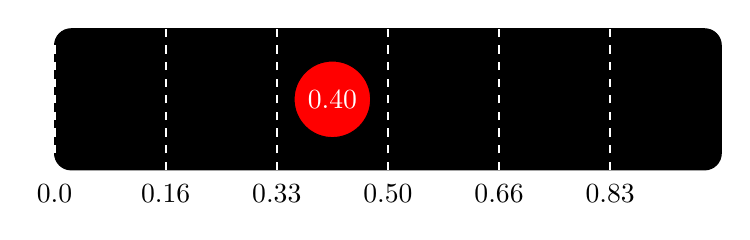
\begin{tikzpicture}
    \usetikzlibrary{shapes.misc, positioning, svg.path}
    
    \fill [black,draw]
  {[rounded corners=6](0,0) --
  ++(\trillWidth, 0)  --
  ++(0, \trillHeight) --
  ++(-\trillWidth, 0) --
  cycle
  {}};

  \draw[white, thick, dashed] (0, 0) -- (0 ,\trillHeight);
  \draw[white, thick, dashed] (\StringWidth*1, 0) -- (\StringWidth*1 ,\trillHeight);
  \draw[white, thick, dashed] (\StringWidth*2, 0) -- (\StringWidth*2 ,\trillHeight);
  \draw[white, thick, dashed] (\StringWidth*3, 0) -- (\StringWidth*3 ,\trillHeight);
  \draw[white, thick, dashed] (\StringWidth*4, 0) -- (\StringWidth*4 ,\trillHeight);
  \draw[white, thick, dashed] (\StringWidth*5, 0) -- (\StringWidth*5 ,\trillHeight);
  
   %\draw[white, thick, dashed] (0, 0) -- (0 ,\trillHeight);
   \node[align=left] at (\StringWidth*0, -0.3) {0.0};
   \node[align=left] at (\StringWidth*1, -0.3) {0.16};
   \node[align=left] at (\StringWidth*2, -0.3) {0.33};
   \node[align=left] at (\StringWidth*3, -0.3) {0.50};
   \node[align=left] at (\StringWidth*4, -0.3) {0.66};
   \node[align=left] at (\StringWidth*5, -0.3) {0.83};
   
   \node[draw,circle, fill=red, text=white] at (\StringWidth/2 + \StringWidth*2,\trillHeight/2) {0.40};

    \end{tikzpicture}
    \caption{Demonstration of the sensor boundaries $\mathbf{B}_n$ for N=6. The vertical dashed lines represent the string boundaries $\mathbf{B}_n$, \textit{not} digital strings. }
    \label{fig:my_label}
\end{figure}